\section{Empirical Portfolio Learnability}
\label{sec:empirics}

\subsection{Data, Representation, and Investment Performance}

The empirical exercise asks how a representation of stock characteristics,
finite return history, and regularization jointly shape a portfolio policy.
A richer representation makes additional portfolio opportunities available,
but a finite return history does not necessarily make all those opportunities
learnable or financially valuable. We first compare Linear, Gaussian, and
Mat\'ern-$3/2$ policies on identical subsequent months. We then fix the Gaussian
representation to examine regularization and the economic content of its
additional directions. The evidence is descriptive historical evidence:
neither a favorable Sharpe nor an estimated number of active directions
certifies a reliably profitable opportunity.

We use the monthly U.S. equity characteristic panel of Jensen, Kelly, and
Pedersen, with formations from January 1963 through December 2024. Starting
from their research dictionary, we exclude nano stocks, retain the 130
characteristics with greatest coverage in 1963--1972, and remove observations
missing more than 30\% of these inputs. Observed values receive average
cross-sectional ranks on $[-0.5,0.5]$; remaining missing inputs receive zero.
The panel is unbalanced. The retrospectively constructed characteristic
dictionary and current data snapshot constitute the academic information set,
rather than a reconstruction of historical signal discovery or data vintages.

There is a material sample limitation. Unavailable subsequent payoffs are
excluded before ranking and calculating the number of stocks $N_t$. A
formation-only audit leaves \MissingCount\ unidentified stock-month payoffs out
of \FormationCount\ eligible observations (\MissingShare\%); documented
adjacent-calendar source matches recover none. Formation-only ranks are
invariant to perturbing future payoff availability, whereas the retained
complete-payoff sample is conditional on that availability. Thus selection
uses only earlier observed payoff values, but sample formation still depends
on whether future payoffs are available. Unknown returns are never assigned
zero. All performance and cost results retain this caveat.

The first inner training period uses 1963--1972 formations and validation
uses 1973--1977. Each subsequent January-close decision reserves the preceding
60 formation months for validation, then refits on the full available
pretest history. December's payoff is known at January close. January--December
formation positions therefore realize February--next January returns. All three
policies are evaluated on the same 564 OOS months, February 1978--January 2025.

Linear uses a constant and the characteristic coordinates. Gaussian and
Mat\'ern-$3/2$ use 10,000 random Fourier features with seed 0. For each kernel,
chronological validation jointly selects lengthscale and ridge penalty by
minimizing the mean response-one quadratic loss $Q$ at fitted scale.
Lengthscales are $\{0.25,0.5,1,2,4\}$ times the initial-sample median distance;
each has 120 penalties fixed from its own initial training spectrum. Frequency
and phase draws are shared across lengthscales. The chosen pair is refitted
using training and validation observations before the test year; no test
payoff selects either parameter. Linear selects its penalty by the same
chronological loss criterion. This is a comparison of representations under
past validation; finite feature banks do not establish strict nesting or
identify a population approximation gap from an observed performance ranking.

\begin{figure}[!htbp]
\centering
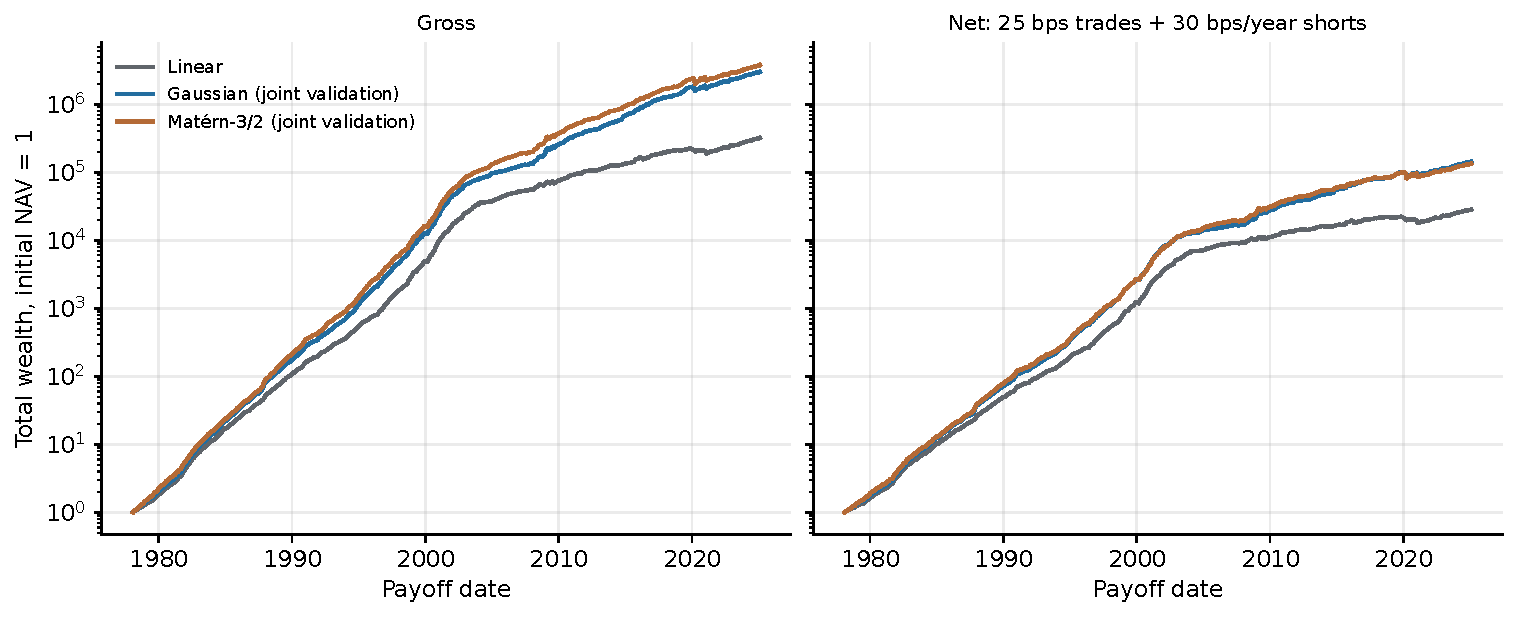
\includegraphics[width=\textwidth]{figures/fig03_representation_wealth.pdf}
\caption{Investment performance on identical OOS months. Linear validates
its ridge penalty; Gaussian and Mat\'ern-$3/2$ jointly validate lengthscale and
penalty using earlier observations. Total wealth compounds cash returns plus
portfolio excess payoffs, starting from NAV one at January 1978 close. The
right panel applies 25-basis-point commissions to both purchases and sales
against drift-adjusted holdings, plus a 30-basis-point annual short fee.
These are illustrative costs on a sample conditional on future-payoff availability.}
\label{fig:equity_kernels}
\end{figure}

\begin{table}[!htbp]\centering\small\setlength{\tabcolsep}{5pt}
\caption{Representation comparison under chronological validation}\label{tab:kernel_performance}
\begin{tabular}{@{}lrrrrrrr@{}}\toprule
Policy & Mean \% & Vol. \% & $\mathrm{SR}_G$ & $\mathrm{SR}_N$ & Gross & Trades & Fees \% \\ \midrule
Linear & 23.44 & 7.58 & 3.091 & 2.476 & 2.01 & 19.45 & 5.14 \\
Gaussian & 28.34 & 7.77 & 3.646 & 2.857 & 2.44 & 24.53 & 6.48 \\
Mat\'ern-$3/2$ & 28.85 & 8.04 & 3.587 & 2.747 & 2.58 & 26.82 & 7.07 \\
\bottomrule\end{tabular}\par\vspace{5pt}
\begin{minipage}{\textwidth}\footnotesize All policies use the same 564 months, February 1978--January 2025, and common initial-validation exposure scale. Gaussian and Mat\'ern jointly validate lengthscale and penalty; Linear validates penalty. Mean and volatility are annualized gross excess returns. Net Sharpe applies 25 bps two-sided commissions and 30 bps/year short fees. Gross is mean account gross/NAV; trades are annual drift-adjusted traded notional/NAV on the net path; fees are annual trading plus short charges/NAV. Costs are illustrative assumptions.\end{minipage}\end{table}


A common positive scale, \PortfolioScale, maps the initial Linear validation
policy's median gross exposure to 1.8. It is fixed before the first test
payoff and applies to all policies, without future volatility or full-sample
exposure normalization. It leaves gross Sharpe unchanged but matters for
costs. The Gaussian-minus-Linear gross Sharpe difference is \KernelGrossDelta,
with paired 12-month-block interval [\KernelGrossLow,\KernelGrossHigh]; the
net difference is \KernelNetDelta, with interval
[\KernelNetLow,\KernelNetHigh]. The corresponding Mat\'ern differences are
\MaternGrossDelta\ [\MaternGrossLow,\MaternGrossHigh] gross and
\MaternNetDelta\ [\MaternNetLow,\MaternNetHigh] net. These comparisons condition
on the fitted paths and use the same resampled months for each policy. Trading
requirements and uncertainty accompany the point estimates; the comparison
does not establish uniform dominance of one representation.

\subsection{A Fixed Economic Spectrum and Active Complexity}

For the remainder of the section we use the existing fixed-lengthscale Gaussian
specification: initial median distance \FixedLengthscale, 10,000 seed-0 features,
and the original past-validation ridge selections. Its full-policy gross/net
Sharpes are \FixedGrossSR/\FixedNetSR. These are distinct from the jointly
validated Gaussian returns in Figure~\ref{fig:equity_kernels} and
Table~\ref{tab:kernel_performance}. Fixing lengthscale and feature draws keeps
the opportunity representation unchanged: varying $\lambda$ then changes
regularization within the same managed-payoff operator. A lengthscale change
would alter both that operator and the portfolios being decomposed.

Let $G$ contain historical monthly managed payoffs
$X_t=N_t^{-1}\sum_i R^e_{i,t+1}\phi(Z_{i,t})$. Response-one ridge fits
$a_\lambda=(G'G/T+\lambda I)^{-1}G'\mathbf{1}/T$ for positive $\lambda$.
The uncentered second-moment spectrum of $G'G/T$ orders directions by
historical payoff variation. An eigenvalue is neither invested capital,
expected return, Sharpe, nor a uniquely named anomaly.
Figure~\ref{fig:spectrum_2024} uses only the history available at January
2024 close. Raw eigenvalues preserve representation units; division by the
trace is a concentration diagnostic that does not rescale the fitted policy.

\begin{figure}[!htbp]
\centering
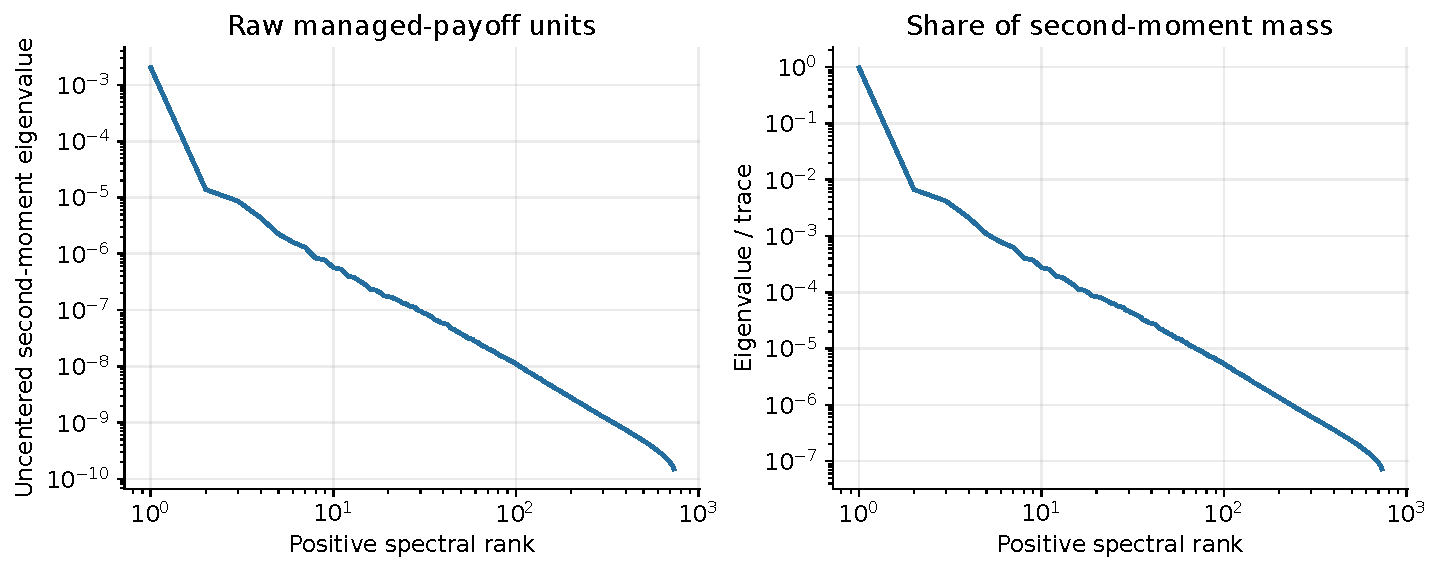
\includegraphics[width=\textwidth]{figures/fig04_fixed_gaussian_spectrum.pdf}
\caption{Managed-payoff spectrum of the fixed Gaussian representation at
January 2024 close. Formations through December 2023 give 732 known monthly
payoffs. The left panel shows raw uncentered second-moment eigenvalues; the
right divides by their trace. Both use the same fixed initial median
lengthscale and feature bank as Figures~\ref{fig:complexity_gaussian}--\ref{fig:economic_holdings}
and the spectral accounts in Table~\ref{tab:spectral_value}.}
\label{fig:spectrum_2024}
\end{figure}

Mass concentration and active complexity are distinct. Ridge weights a
direction by $\widehat\mu_j/(\widehat\mu_j+\lambda)$, giving
$C(\lambda)=\sum_j\widehat\mu_j/(\widehat\mu_j+\lambda)$. Weak eigenvalues can
contribute many effective degrees of freedom while carrying little
second-moment mass. Across annual histories, the first 10\% of positive
Gaussian ranks contain \LeadingMass\% of mass, but contribute only
\LeadingComplexity\ of the selected policy's \TotalComplexity\ mean effective
directions. Positive rank uses a relative $10^{-12}$ eigenvalue tolerance;
near-tied eigenvalues are kept together at group boundaries. Feasible
complexity cannot exceed this historical effective rank, which is at most
the number of historical monthly observations. A long weak tail can change
exposures without establishing that its opportunities are learnable.

\begin{figure}[!htbp]
\centering
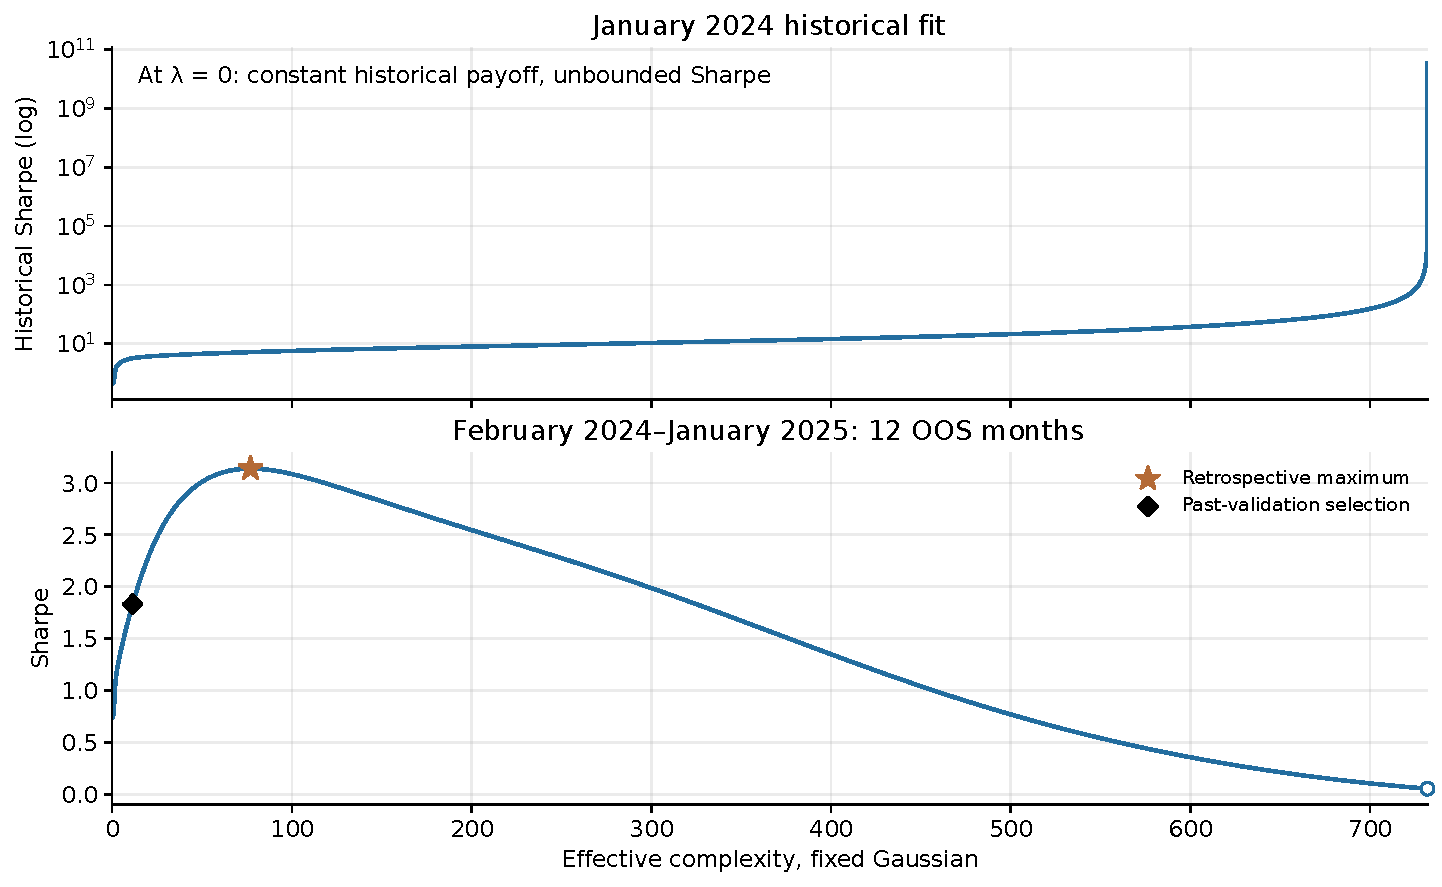
\includegraphics[width=\textwidth]{figures/fig05_fixed_gaussian_2024.pdf}
\caption{Complete regularization path for the fixed Gaussian January 2024
refit. Historical Sharpe uses a logarithmic scale; subsequent Sharpe uses a
separate linear scale. Exact response-one interpolation has zero historical
variance and unbounded historical Sharpe; unresolved numerical ratios near
that limit are omitted from the historical panel only.
Each positive-penalty point is evaluated on its actual February
2024--January 2025 OOS payoffs. The open circle is the exact minimum-norm
zero-penalty policy at effective rank 732. The star is the retrospective
maximum over the extended evaluation grid; the diamond retains the original
earlier-validation selection. Neither is an estimate of a significant population optimum.}
\label{fig:complexity_gaussian}
\end{figure}

The final-year path holds lengthscale, feature bank, and history fixed. Its
retrospective maximum is at complexity \SinglePeakC\ with subsequent Sharpe
\SinglePeakSR; at zero penalty Sharpe is \SingleZeroSR. Historical fit and
subsequent investment performance need not move together. Twelve subsequent
months produce a noisy illustration, so Figure~\ref{fig:complexity_nine}
provides the complete progression in nine historical blocks.

The evaluation grid retains every original penalty and adds a logarithmic
sequence from strong regularization to very small positive penalties, followed
by exactly $\lambda=0$. Its \CandidateCount\ policies are evaluated separately
at every annual refit. The zero endpoint uses a symmetric eigensystem
Moore--Penrose pseudoinverse with the same positive-rank tolerance, rather than
an inverse of a singular operator. Direct feature-space least squares checks
the first and final endpoints, and the smallest positive penalties converge
numerically to the zero returns. No added evaluation changes the original
validation policy, and no OOS result selects a deployable penalty.

To assess the historical Sharpe--complexity trade-off using year-specific
effective complexity rather than block-average complexity,
Figure~\ref{fig:complexity_nine} reports one representative annual profile
from each of the nine historical blocks. We select the central calendar
year in each block: 1980, 1985, 1990, 1995, 2000, 2005, 2010, 2015, and
2021. Holding the Gaussian representation and lengthscale fixed, each
profile connects the full evaluated penalty path using that year's
effective complexity and the annualized Sharpe of its 12 subsequent
monthly OOS returns. The annual past-validation selection is therefore
an actual point on its own annual curve. These one-year profiles are
noisier than pooled-block profiles and their retrospective maxima are
descriptive. The historical table and block summaries below retain the
original pooled-block results.

\begin{figure}[!htbp]
\centering
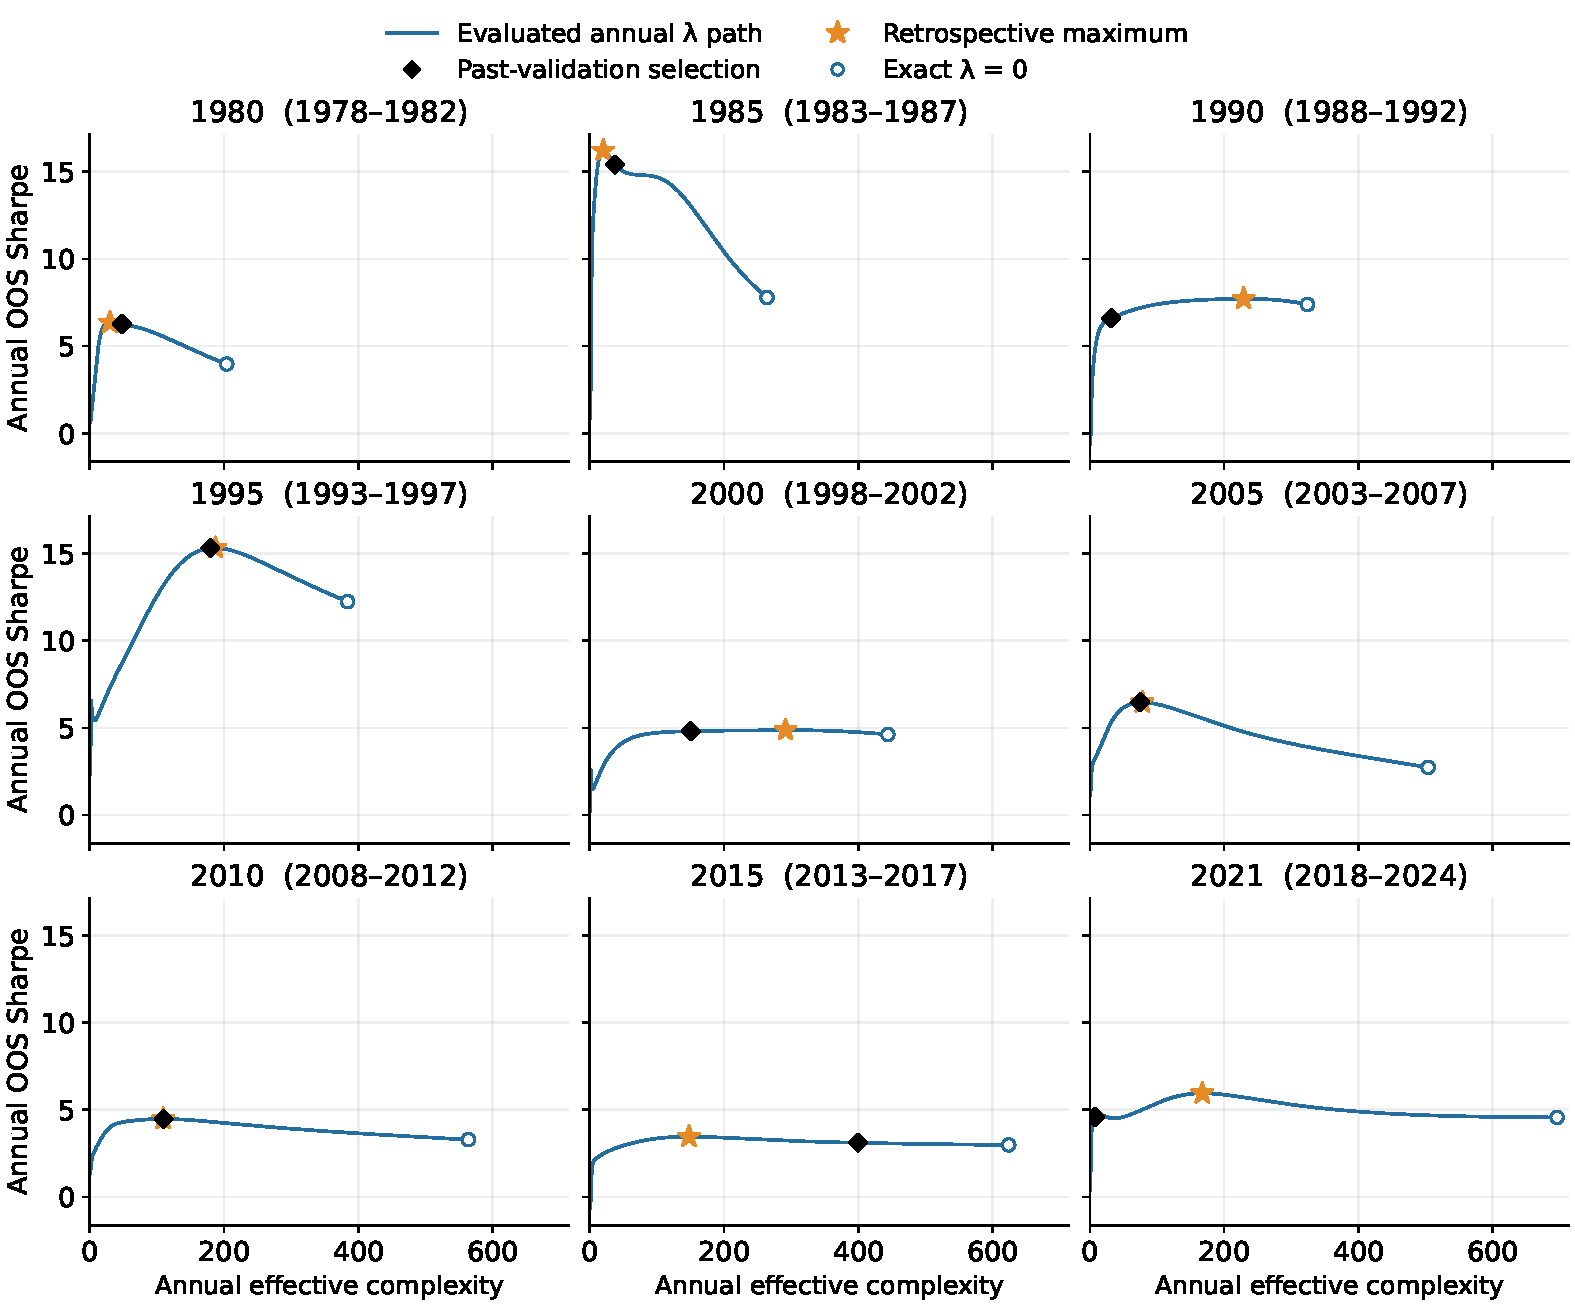
\includegraphics[width=\textwidth]{figures/fig06_nine_complete_profiles.pdf}
\caption{Representative annual out-of-sample Sharpe--complexity profiles.
Each panel corresponds to one selected decision year, the central calendar
year of its indicated historical block: 1980, 1985, 1990, 1995, 2000,
2005, 2010, 2015, or 2021. Annual OOS Sharpe is annualized from the 12
subsequent monthly returns (February of the decision year through January
of the following year); effective complexity is measured for that same
year's fitted policy, with no averaging across years or pooling of returns.
The Gaussian representation and lengthscale are fixed. Curves connect all
actual evaluated penalties, including the extended near-zero positive
grid and the exact minimum-norm $\lambda=0$ endpoint, without smoothing
or extrapolation. Black diamonds mark annual past-validation selections
verified to lie on their annual curves; orange stars mark retrospective
maxima over the full annual evaluated grid; open circles mark exact
zero-penalty endpoints. All nine panels share common axes. These profiles
are noisier than the previous pooled-block curves because each uses only
one OOS year. Retrospective maxima do not select deployable policies or
estimate population-optimal complexity.}
\label{fig:complexity_nine}
\end{figure}

\begin{table}[!htbp]\centering\small\setlength{\tabcolsep}{5pt}
\caption{Annual retrospective maxima and exact unregularized endpoints}
\label{tab:historical_endpoints}
\begin{tabular}{@{}lrrrrr@{}}\toprule
Decision year & $C$ at max. & Max. SR & $C(0)$ & SR at $\lambda=0$ & Decline \\ \midrule
1980 & 30.0 & 6.355 & 204 & 3.971 & 2.384 \\
1985 & 20.0 & 16.209 & 264 & 7.785 & 8.424 \\
1990 & 229.0 & 7.718 & 324 & 7.385 & 0.333 \\
1995 & 187.2 & 15.320 & 384 & 12.239 & 3.081 \\
2000 & 291.5 & 4.874 & 444 & 4.622 & 0.252 \\
2005 & 78.3 & 6.470 & 504 & 2.736 & 3.734 \\
2010 & 109.3 & 4.474 & 564 & 3.285 & 1.189 \\
2015 & 147.6 & 3.460 & 624 & 2.984 & 0.476 \\
2021 & 167.5 & 5.945 & 696 & 4.563 & 1.382 \\
\bottomrule\end{tabular}\par\vspace{5pt}
\begin{minipage}{\textwidth}\footnotesize
The decision years are the same nine selected years as in Figure~\ref{fig:complexity_nine}.
Each maximum uses the full annual evaluated grid, including the exact $\lambda=0$ endpoint.
Sharpe is annualized from the 12 subsequent monthly OOS returns; complexity is measured
for that same annual fit, without averaging across years. $C(0)$ is the annual
historical effective rank. Decline is maximum minus zero-penalty Sharpe,
a descriptive change rather than a significance test.
\end{minipage}\end{table}


\HistoricalFindings
These are descriptive shapes, not evidence of a statistically identified
optimum in every period. Broad regions can be nearly flat relative to sampling
uncertainty. All displayed maxima have been
recomputed on the extended grid, including zero.

Intervals use 5,000 paired circular-block resamples, sharing monthly draws
across all candidates or contrasted portfolios. They condition on estimated
policies, representations, and holdings; they do not repeat model selection.
Approximate stability and dependence decay within a block motivate this
diagnostic. It neither corrects for searching the grid nor establishes
validity under arbitrary nonstationarity. Six- and 24-month-block results for
the representation comparisons and economic contrasts accompany the canonical
results. A favorable retrospective peak is consequently distinct from a
learnable policy selected using past information.

\subsection{What Additional Directions Trade}

We interpret portfolios associated with eigenspaces of the same fixed
Gaussian policy. At each annual refit, four disjoint positive-rank groups
partition its ridge coefficients. Their actual contributions are reconstructed
as stock-level signed holdings, providing long and short characteristic
profiles and subsequent payoff and covariance attribution. The same selected
penalty is retained across nested comparisons. These are attribution
portfolios within one policy, not independently optimized strategies.
Near-tied eigenvectors can rotate, so group profiles carry the historical
interpretation rather than persistent names assigned to individual eigenvectors.

\begin{figure}[!htbp]
\centering
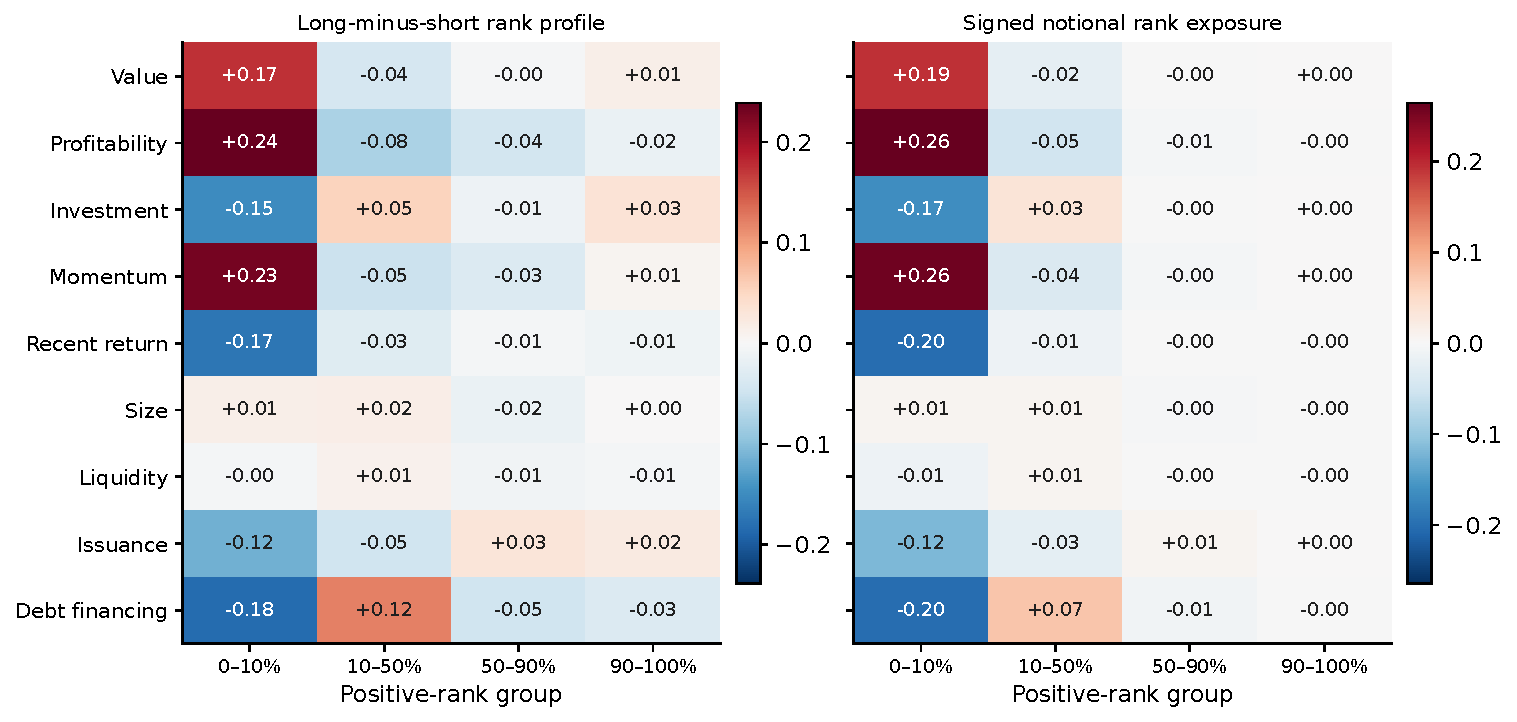
\includegraphics[width=\textwidth]{figures/fig07_fixed_gaussian_holdings.pdf}
\caption{Economic profiles of the fixed Gaussian policy's actual spectral
holdings. The left panel gives long-minus-short weighted formation-rank
scores; the right preserves investment scale through signed notional
exposures. An explicit signed characteristic dictionary defines the families.
Debt financing and equity issuance are distinct. Families can overlap and
cannot be added as disjoint return components. These holdings decompose the
fixed representation, independently of the tuned-kernel opening comparison.}
\label{fig:economic_holdings}
\end{figure}

Leading holdings favor profitability and oppose recent returns and debt
financing. Intermediate directions modify those exposures within the same
characteristic universe. A large normalized characteristic contrast can
coexist with small notional exposure, so profiles and signed notionals answer
different questions. Formation descriptors characterize what is held;
subsequent outcomes determine its investment contribution.

\begin{table}[!htbp]\centering\small\setlength{\tabcolsep}{5pt}
\caption{Fixed Gaussian spectral groups and incremental investment value}\label{tab:spectral_value}
\begin{tabular}{@{}lrrrrrr@{}}\toprule
Ranks & Mass \% & Own gross & Account gross & Mean \% & $\mathrm{SR}_G$ & $\mathrm{SR}_N$ \\ \midrule
0--10\% & 99.9215 & 2.267 & 2.267 & 24.323 & 3.012 & 2.354 \\
10--50\% & 0.0685 & 1.263 & 2.333 & 2.759 & 3.284 & 2.598 \\
50--90\% & 0.0091 & 0.327 & 2.325 & 0.047 & 3.286 & 2.594 \\
90--100\% & 0.0010 & 0.078 & 2.326 & 0.026 & 3.300 & 2.605 \\
\bottomrule\end{tabular}\par\vspace{5pt}
\par\vspace{9pt}\begin{tabular}{@{}lrrrr@{}}\toprule
Added ranks & $\Delta Q$ & Cross term & Own square & Paired 95\% interval \\ \midrule
0--10\% & -0.402340 & -1.083912 & 0.681573 & [-0.524808, -0.257425] \\
10--50\% & -0.036008 & -0.131766 & 0.095758 & [-0.093264, +0.027912] \\
50--90\% & +0.000168 & -0.003978 & 0.004146 & [-0.008734, +0.009000] \\
90--100\% & -0.003123 & -0.003547 & 0.000424 & [-0.006796, -0.000185] \\
\bottomrule\end{tabular}\par\vspace{5pt}
\begin{minipage}{\textwidth}\footnotesize The original selected penalty is retained at each annual refit. Mass averages annual historical second-moment shares. Own gross and mean describe individual components; account gross and Sharpes describe all groups through that boundary. The lower panel reports raw fitted-scale loss changes, relative to the null portfolio for the first group, with the same 5,000 paired 12-month-block draws. Weights are summed at stock level before trades and short fees. Gross Sharpe increments are +0.272, +0.002, +0.014; net increments are +0.244, -0.004, +0.011.\end{minipage}\end{table}


The leading group has mean component gross \LeadingGross\ and annual excess
payoff \LeadingMean\%. Adding intermediate directions contributes
\IntermediateMean\% annually. Their own gross \IntermediateGross\ increases
the cumulative account's gross by only \IncrementalGross: some added positions
offset existing stock holdings. Component gross exposures therefore do not
add to the combined account's gross. The component's annual covariance with
the leading portfolio is \IntermediateCovariance, while total annual variance
changes by \IntermediateVariance. Negative covariance can coexist with
increased account variance because the component also adds its own variance.

Gross Sharpe rises from \LeadingSR\ to \TwoGroupSR, and net Sharpe from
\LeadingNetSR\ to \TwoGroupNetSR. Paired 12-month-block intervals for these
changes are [\GroupGrossLow,\GroupGrossHigh] and
[\GroupNetLow,\GroupNetHigh]. The response-one loss changes by \IntermediateQDelta,
with interval [\IntermediateQLow,\IntermediateQHigh]; its cross term is
\IntermediateQCross\ and own-square term \IntermediateQSquare. Thus a positive
standalone mean, a Sharpe increment, and an incremental $Q$ improvement are
distinct assessments. The incremental identity
$\Delta Q=-2\,\overline{(1-P)A}+\overline{A^2}$ includes the interaction of
the previous policy $P$ and added payoff $A$, at their original fitted scale.

Small incremental account gross does not imply small turnover. Monthly
characteristics and annual refits can change offsetting positions substantially.
For every nested account, stock weights are summed before calculating trades
against drift-adjusted holdings, short notional, and net returns. Costs begin
with entry from cash. Target weights refer to post-execution NAV; proportional
commissions are solved jointly with the target cash residual. The annual
short fee is divided by twelve. Cash earns or pays the same monthly risk-free
rate, and terminal holdings are marked rather than forcibly liquidated.
Separate component fees would not reconstruct the netted account. Changes in
target weights remain a separate turnover proxy, never observed execution costs.

Corporate-action and delisting treatment relies on the upstream JKP return
construction and stable identifiers; there is no independent share-count or
execution-tape reconstruction. Liquidated names incur trades but receive no
invented next payoff. The cost assumptions omit market impact and additional
funding spreads. They are self-financing friction sensitivities, with the
same future-payoff-availability caveat as gross returns.

The weak tail has little historical second-moment mass and small absolute
payoff contributions. The successive gross/net Sharpe increments in
Table~\ref{tab:spectral_value} include adverse as well as favorable outcomes;
the loss decomposition also retains the own-square and cross terms. Small
mass alone cannot rule out covariance value, while a striking normalized
characteristic tilt need not have a material financial contribution.
Six-benchmark regressions of the actual component returns give descriptive
spanning statistics; a separate hedge uses only pretest slope estimates.
Neither supplies an independently selected investment strategy or a newly
identified risk premium.

Economic content and supported complexity vary with history. The stationary
theory is a benchmark for approximately stable conditions; a local
interpretation requires those conditions. Descriptive complexity changes do
not identify a population spectral-decay parameter. Across the representation
comparison, fixed-kernel regularization paths, and stock-level attribution,
the financial question is whether additional available directions improve
the portfolio that finite historical information can support.
